\begin{figure}[H]
	\centering
	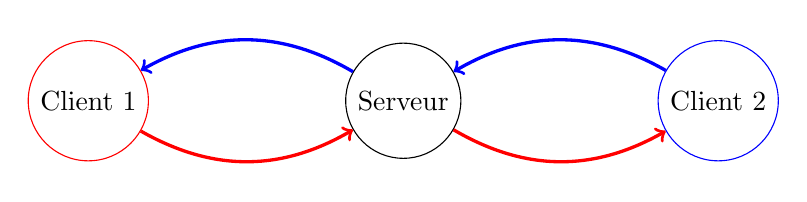
\begin{tikzpicture}
		\begin{scope}[every node/.style={circle, draw}]
			\node (S) at (0,0) {Serveur};
			\node[draw=red] (C1) at (-4,0) {Client 1};
			\node[draw=blue] (C2) at (4,0) {Client 2};
		\end{scope}
		\begin{scope}[every edge/.style={draw=red, very thick, bend right=30}]
			\path [->] (C1) edge node {} (S);
			\path [->] (S) edge node {} (C2);
		\end{scope}
		\begin{scope}[every edge/.style={draw=blue, very thick, bend right=30}]
			\path [->] (C2) edge node {} (S);
			\path [->] (S) edge node {} (C1);
		\end{scope}
	\end{tikzpicture}
	\caption{Une représentation abstraite du modèle client-serveur}
	\label{fig:repr-serveur}
\end{figure}

Le modèle client serveur implique deux choses.
Premièrement, il est nécessaire d'isoler les responsabilités entre le module client et le module serveur.
Secondement, il est nécessaire d'avoir une interface pour que les modules puissent communiquer.
Cette dernière est imposée par le sujet.

\subsection{Isolation des responsabilités}

Le serveur est responsable du lancement, du déroulement, ainsi que la terminaison de la partie.
Le client est responsable des coups qu'il joue lorsque le serveur lui demande de jouer, 
en l'informant du coup de son adversaire au tour précédent.

On remarque que les deux modules ont besoin de pouvoir garder en mémoire l'évolution d'une partie.
Le serveur en a besoin pour savoir si un joueur fait un coup invalide.
Les clients en ont besoin pour suivre une stratégie cohérente.

On décide de faire un troisième module nommé Common qui implémentera toutes les fonctionnalités communes 
aux clients et au serveur.

\subsection{Interface entre client et serveur}

Les clients doivent disposer de quatres fonctions.
\begin{itemize}
    \item \textbf{get\_player\_name()} : Retourne le nom du joueur.
    \item \textbf{initialize()} : Permet au joueur de se prépaprer pour la partie à venir.
    \item \textbf{play(coup\_precedent)} : Demande au joueur un coup, en fonction 
    du coup fait par son adversaire au tour précédent.
    \item \textbf{finalize()} : Permet au joueur de libérer les ressources allouées.
\end{itemize}

Cette interface établie une généricité entre tous les clients et permet de les faire s'affronter.
Cela rend possible la création d'une compétition pour établir quelle est 
la meilleur stratégie.